\documentclass[submit]{harvardml}

\course{CS181-S22}
\assignment{Assignment \#4}
\duedate{11:59pm EST, March 25, 2022} 

\usepackage[OT1]{fontenc}
\usepackage[colorlinks,citecolor=blue,urlcolor=blue]{hyperref}
\usepackage[pdftex]{graphicx}
\usepackage{graphicx}
\usepackage{caption}
\usepackage{fullpage}
\usepackage{soul}
\usepackage{amsmath}
\usepackage{framed}
\usepackage{amssymb}
\usepackage{color}
\usepackage{todonotes}
\usepackage{listings}
\usepackage{common}
\usepackage{physics}
\usepackage{amsmath}
\usepackage{pythonhighlight}

\usepackage[mmddyyyy,hhmmss]{datetime}

\definecolor{verbgray}{gray}{0.9}

\lstnewenvironment{csv}{
  \lstset{backgroundcolor=\color{verbgray},
  frame=single,
  framerule=0pt,
  basicstyle=\ttfamily,
  columns=fullflexible}}{}
 
\begin{document}

\begin{center}
{\Large Homework 4: SVM, Clustering, and Ethics}\\
\end{center}

\subsection*{Introduction}

This homework assignment will have you work with SVMs, 
clustering, and engage with the ethics lecture.  We encourage you to
read Chapters 5 and 6 of the course textbook.

Please submit the \textbf{writeup PDF to the Gradescope assignment `HW4'}. Remember to assign pages for each question.

Please submit your \textbf{\LaTeX\ file and code files to the Gradescope assignment `HW4 - Supplemental'}. 

\newpage

%%%%%%%%%%%%%%%%%%%%%%%%%%%%%%%%%%%%%%%%%%%%%
% Problem 1
%%%%%%%%%%%%%%%%%%%%%%%%%%%%%%%%%%%%%%%%%%%%%
\begin{problem}[Fitting an SVM by hand, 10pts]

  For this problem you will solve an SVM by hand, relying on principled rules and SVM properties. 
  For making plots, however, you are allowed to use a computer or other graphical tools.

Consider a dataset with the following 7 data points each with $x \in \reals$ and $y \in \{ -1, +1 \}$ : \[\{(x_i, y_i)\}_{i = 1}^7 =\{(-3 , +1) , (-2 , +1 ) , (-1,  -1 ), (0, +1), ( 1 , -1 ), ( 2 , +1 ) , (3 , +1 )\}\] Consider
mapping these points to $2$ dimensions using the feature vector $\bphi(x) =  (x, -\frac{8}{3}x^2 + \frac{2}{3}x^4 )$. The hard margin classifier training problem is:
%
\begin{align*}
  &\min_{\mathbf{w}, w_0} \frac{1}{2}\|\mathbf{w}\|_2^2 \label{eq:dcp} \\
  \quad \text{s.t.} \quad & y_i(\mathbf{w}^\top \bphi(x_i) + w_0) \geq 1,~\forall i \in \{1,\ldots, n\}\notag
\end{align*}

Make sure to follow the logical structure of
the questions below when composing your answers, and to justify each step.

\begin{enumerate}
\item Plot the transformed training data in $\reals^2$ and draw the
  optimal decision boundary of the max margin classifier. You can
  determine this by inspection (i.e. by hand, without actually doing
  any calculations).

\item What is the value of the margin achieved by the optimal decision
  boundary found in Part 1?

\item Identify a unit vector that is orthogonal to the decision boundary.

\item Considering the discriminant
  $h(\bphi(x);\boldw,w_0)=\boldw^\top\bphi(x) +w_0$, give an
  expression for {\em all possible} $(\boldw,w_0)$ that define the
  optimal decision boundary from 1.1.  Justify your answer.

  Hint: The boundary is where the discriminant is equal to 0.  Use
  what you know from 1.1 and 1.3 to solve for $\boldw$ in terms of
  $w_0$.  (If you solve this problem in this way, then $w_0$
  corresponds to your free parameter to describe the set of all
  possible $(\boldw,w_0)$.)
  
\item Consider now the training problem for this dataset. Using your
  answers so far, what particular solution to $\boldw$ will be optimal
  for the optimization problem?

\item What is the corresponding optimal value of $w_0$ for the
  $\boldw$ found in Part 5 (use your result from Part 4 as guidance)?
  Substitute in these optimal values and write out the discriminant
  function $h(\bphi(x);\boldw,w_0)$ in terms of the variable $x$ .


\item Which points could possibly be support vectors of the classifier?  Confirm that
  your solution in Part 6 makes the constraints above tight---that is,
  met with equality---for these candidate points.

\item Suppose that we had decided to use a different feature mapping
    $\bphi'(x) = (x, -\frac{31}{12}x^2 + \frac{7}{12}x^4 )$.  Does
    this feature mapping still admit a separable solution?  How does
    its margin compare to the margin in the previous parts?  Based on
    this, which set of features might you prefer and why? 
    
\end{enumerate}

\end{problem}

\newpage
\subsection*{Solution}

\subsection*{1.1}

We want to plot the transformed training data and draw the optimal decision boundary of the max margin classifier.

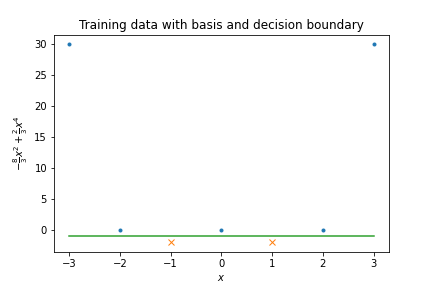
\includegraphics{plots/1-1.png}

\subsection*{1.2}

We want to determine the margin achieved by the optimal decision boundary found in Part 1. We know that the margin is the minimum distance between the decision boundary and any data point. As we can see, the distance between the decision boundary and the nearest data point is $1$, and so the \boxed{\text{margin is }$1$}.

\subsection*{1.3}

As we can see from 1.1, the decision boundary is horizontal line. So a unit vector that is orthogonal to the decision boundary is $\boxed{\vb{u} =[0, 1]}$.

\subsection*{1.4}

We want to give an expression for all possible $(\vb{w}, w_0)$ that define the optimal decision boundary from 1.1. From 1.3 we know that $\vb{w}$ must be some scalar of $\vb{u} = [0, 1]$, so $\textbf{w} = c \vb{u}$. We also know that the boundary is where the discriminant is equal to $0$. Using these facts, we can manipulate the expression from the discriminant.
\begin{align*}
    h(\bphi(x); \vb{w}, w_0) &= \vb{w}^T \bphi(x) + w_0 \\
    0 &= c \vb{u}^T \bphi(x) + w_0 \\
    0 &= c u_1 \phi(x)_1 + c u_2 \phi(x)_2 + w_0 \\
    0 &= c (0) \phi(x)_1 + c (1) \phi(x)_2 + w_0 \\
    c \bphi(x)_2 &= - w_0 \\
\end{align*}
From 1.3 we know that the optimal decision boundary occurs when $\bphi(x)_2 = -1$. And so we have the following expression for $c$
\begin{align*}
    c(-1) &= -w_0 \\
    c &= w_0
\end{align*}
And so since $\textbf{w} = c \vb{u}$ then the optimal decision boundary occurs when $\boxed{\textbf{w} = [0, w_0]}$

\subsection*{1.5}

We want to find the optimal solution $\vb{w}$ using our answers so far. From 1.2 we know that the optimal margin is $1$ and that $\vb{w} = [0, w_0]$. Let us manipulate the training problem.
\begin{align*}
    \min_{\vb{w}, w_0} \frac{1}{2} || \vb{w} ||^2_2 = \min_{\vb{w}, w_0} \frac{1}{2} \vb{w}^T \vb{w} = \min_{\vb{w}, w_0} \frac{1}{2} w_0^2
\end{align*}
By examining the data we see that the only possible $\vb{w}$ that could satisfy the constraints is $\boxed{\vb{w} = [0, 1]}$, which is therefore optimal.

\subsection*{1.6}
We want to find the corresponding optimal value $w_0$ for $\vb{w}$ from Part 1.5. We know from 1.5 that $\vb{w} = [0, 1]$. From 1.4 we know that $\vb{w} = \begin{bmatrix}0 \\ w_0\end{bmatrix}$ and so $w_0 = 1$.

Now we want to substitute in these optimal values and write out the discriminant function in terms of $\vb{w}$.
\begin{align*}
    h(\bphi(x); \vb{w}, w_0) &= \vb{w}^T \bphi(x) + w_0 \\
    h(\bphi(x); \vb{w}, w_0) &= [0, 1]^T \bphi(x) + 1 \\
    h(\bphi(x); \vb{w}, w_0) &= -\frac{8}{3} x^2 + \frac{2}{3} x^4 + 1
\end{align*}

\subsection*{1.7}

The points that could possibly be point vectors of the classifier are $\{ (-2, 1), (-1, -1), (0, 1), (1, -1), (2, 1)$. Let us confirm that the 1.6 solution meets the equality below for these candidate points.
\begin{equation*}
    y_i (\vb{w}^T \bphi(x_i) + w_0) \geq 1, \forall i \in \{1, \dots, n\}
\end{equation*}
We can verify this using the code below.
\begin{python}
support_vectors = np.array([
    [-2, 1],
    [-1, -1],
    [0, 1],
    [1, -1],
    [2, 1]
])
X, y = support_vectors[:,0], support_vectors[:,1]

w, w0 = np.array([[0],[1]]), 1

def basis(x):
    return np.array([x, (-8 / 3) * (x ** 2) + (2 / 3) * (x ** 4)])

def equality(x, y):
    return (y * (np.dot(w.T, basis(x)) + w0)) == 1

np.all([equality(X[i], y[i]) for i in range(y.size)])
\end{python}
This code returns true and so we know that all of the support vectors make the constraints above tight.

\subsection*{1.8}

Supposing we had used a different feature mapping $\bphi'(x) = (x, -4 x^2 + \frac{1}{2} x^4)$, the feature mapping would not admit a separable solution. We can see this in the plot below.

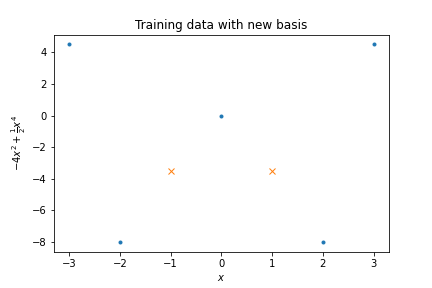
\includegraphics{plots/1-8.png}

Thus we would not be able to find a suitable margin, and so we would prefer the first set of features because it makes the data separable.

\newpage

%%%%%%%%%%%%%%%%%%%%%%%%%%%%%%%%%%%%%%%%%%%%%
% Problem 2
%%%%%%%%%%%%%%%%%%%%%%%%%%%%%%%%%%%%%%%%%%%%%

\begin{problem}[K-Means and HAC, 20pts]

For this problem you will implement K-Means and HAC from scratch to cluster image data. You may use \texttt{numpy} but no third-party ML implementations (eg. \texttt{scikit-learn}).

We've provided you with a subset of the MNIST dataset, a collection of
handwritten digits used as a benchmark for image recognition (learn more at
\url{http://yann.lecun.com/exdb/mnist/}). MNIST is widely used in supervised learning, and modern algorithms do very well. 

You have been given
representations of MNIST images, each of which is a $784\times1$
greyscale handwritten digit from 0-9. Your job is to implement K-means and HAC on MNIST, and to test whether these relatively
simple algorithms can cluster similar-looking images together.

The code in \texttt{T4\_P2.py} loads the images into your environment into two arrays -- \texttt{large\_dataset}, a 5000x784 array, will be used for K-means, while \texttt{small\_dataset}, a 300x784 array, will be used for HAC. In your code, you should use the $\ell_2$ norm (i.e. Euclidean distance) as your distance metric.

\textbf{Important:} Remember to include all of your plots in your PDF submission!

\textbf{Checking your algorithms:} Instead of an Autograder file, we have provided a similar dataset, \texttt{P2\_Autograder\_Data}, and some visualizations, \texttt{HAC\_visual} and \texttt{KMeans\_visual}, for how K-means and HAC perform on this data. Run your K-means (with $K=10$ and \texttt{np.random.seed(2)}) and HAC on this second dataset to confirm your answers against the provided visualizations. Do \textbf{not} submit the outputs generated from \texttt{P2\_Autograder\_Data}. Load this data with \texttt{data = np.load(`P2\_Autograder\_Data.npy')}.

\begin{enumerate}

\item Starting at a random initialization and $K = 10$, plot the
  K-means objective function (the residual sum of squares) as a
  function of iterations and verify that it never increases.

\item For $K=10$ and for 3 random restarts, print the mean image (aka
  the centroid) for each cluster. There should be 30 total images. Code 
  that creates plots for parts 2, 3, and 4 can be found in \texttt{T4\_P2.py}.

\item Repeat Part 2, but before running K-means, standardize or center
  the data such that each pixel has mean 0 and variance 1 (for any
  pixels with zero variance, simply divide by 1). For $K=10$ and 3
  random restarts, show the mean image (centroid) for each
  cluster. Again, present the 30 total images in a single
  plot. Compare to Part 2: How do the centroids visually differ? Why?

\item Implement HAC for min, max, and centroid-based linkages. Fit
  these models to the \texttt{small\_dataset}.  For each of these 3
  linkage criteria, find the mean image for each cluster when using
  $10$ clusters. Display these images (30 total) on a single plot.

  How do the ``crispness'' of the cluster means and the digits
  represented compare to mean images for k-means?  
  Why do we only ask you to run HAC once?  

  \textbf{Important Note:} For this part ONLY, you may use
  \texttt{scipy}'s \texttt{cdist} function to calculate Euclidean
  distances between every pair of points in two arrays.

\item For each of the HAC linkages, as well as one of the runs of your
  k-means, make a plot of ``Number of images in cluster" (y-axis)
  v. ``Cluster index" (x-axis) reflecting the assignments during the
  phase of the algorithm when there were $K=10$ clusters.

  Intuitively, what do these plots tell you about the difference
  between the clusters produced by the max and min linkage criteria?

  Going back to the previous part: How does this help explain the
  crispness and blurriness of some of the clusters?  
\end{enumerate}
\end{problem}

\newpage
\begin{framed}
\noindent\textbf{Problem 2} (cont.)\\
\begin{enumerate}
\setcounter{enumi}{5}
\item For your K-means with $K = 10$ model and HAC min/max/centroid
  models using $10$ clusters on the \texttt{small\_dataset} images,
  use the \texttt{seaborn} module's \texttt{heatmap} function to plot
  a confusion matrix between each pair of clustering methods.  This
  will produce 6 matrices, one per pair of methods. The cell at the
  $i$th row, $j$th column of your confusion matrix is the number of
  times that an image with the cluster label $j$ of one method has
  cluster $i$ in the second method.  Which HAC is closest to k-means?
  Why might that be?

\item Suppose instead of comparing the different clustering methods to
  each other, we had decided to compute confusions of each clustering
  method to the \emph{true} digit labels (you do \emph{not} have to
  actually compute this).  Do you think how well the clustering match
  the true digits is reasonable evaluation metric for the clustering?
  Explain why or why not.
  
\end{enumerate}
\end{framed}


%%%%%%%%%%%%%%%%%%%%%%%%%%%%%%%%%%%%%%%%%%%%%

\newpage
\subsection*{Solution}

\subsection*{2.1}

We want to plot the K-means objective function as a function of iterations and verify that it never increases.

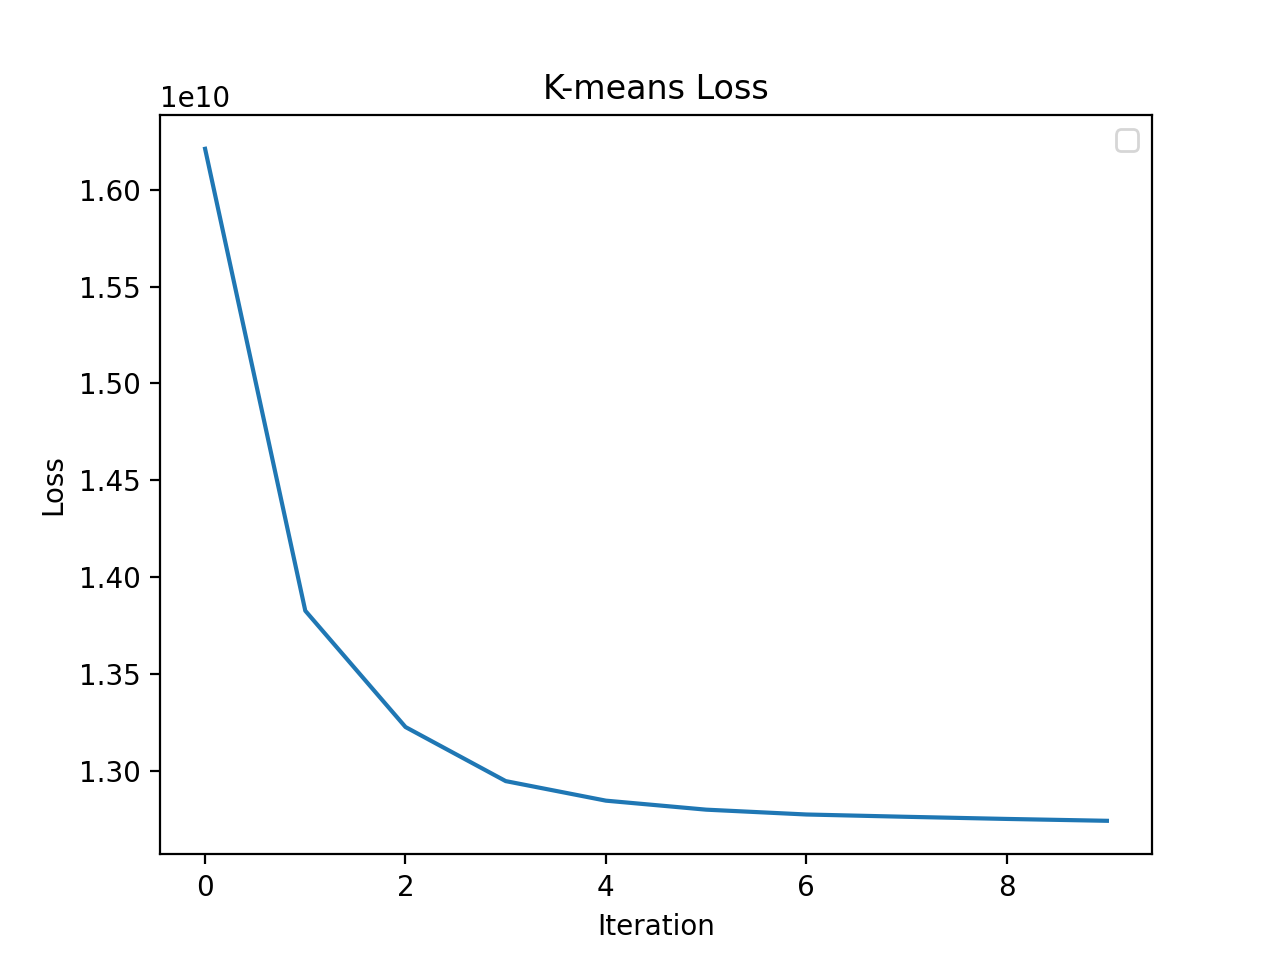
\includegraphics[scale=0.5]{plots/kmeans-loss.png}

As we can see, it never increases.

\newpage
\subsection*{2.2}
We want to show the mean image for each cluster of K-means with $K = 10$ and $3$ random restarts. This is shown in the plot below.

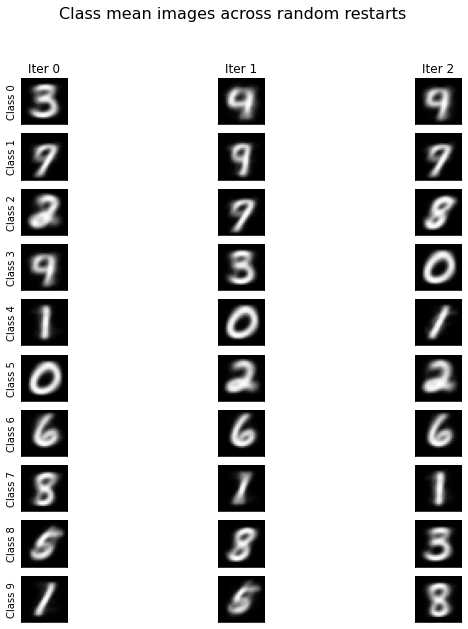
\includegraphics[scale=0.5]{plots/kmeans.png}

\newpage
\subsection*{2.3}
We want to repeat 2.2 but standardize the data before running K-means.

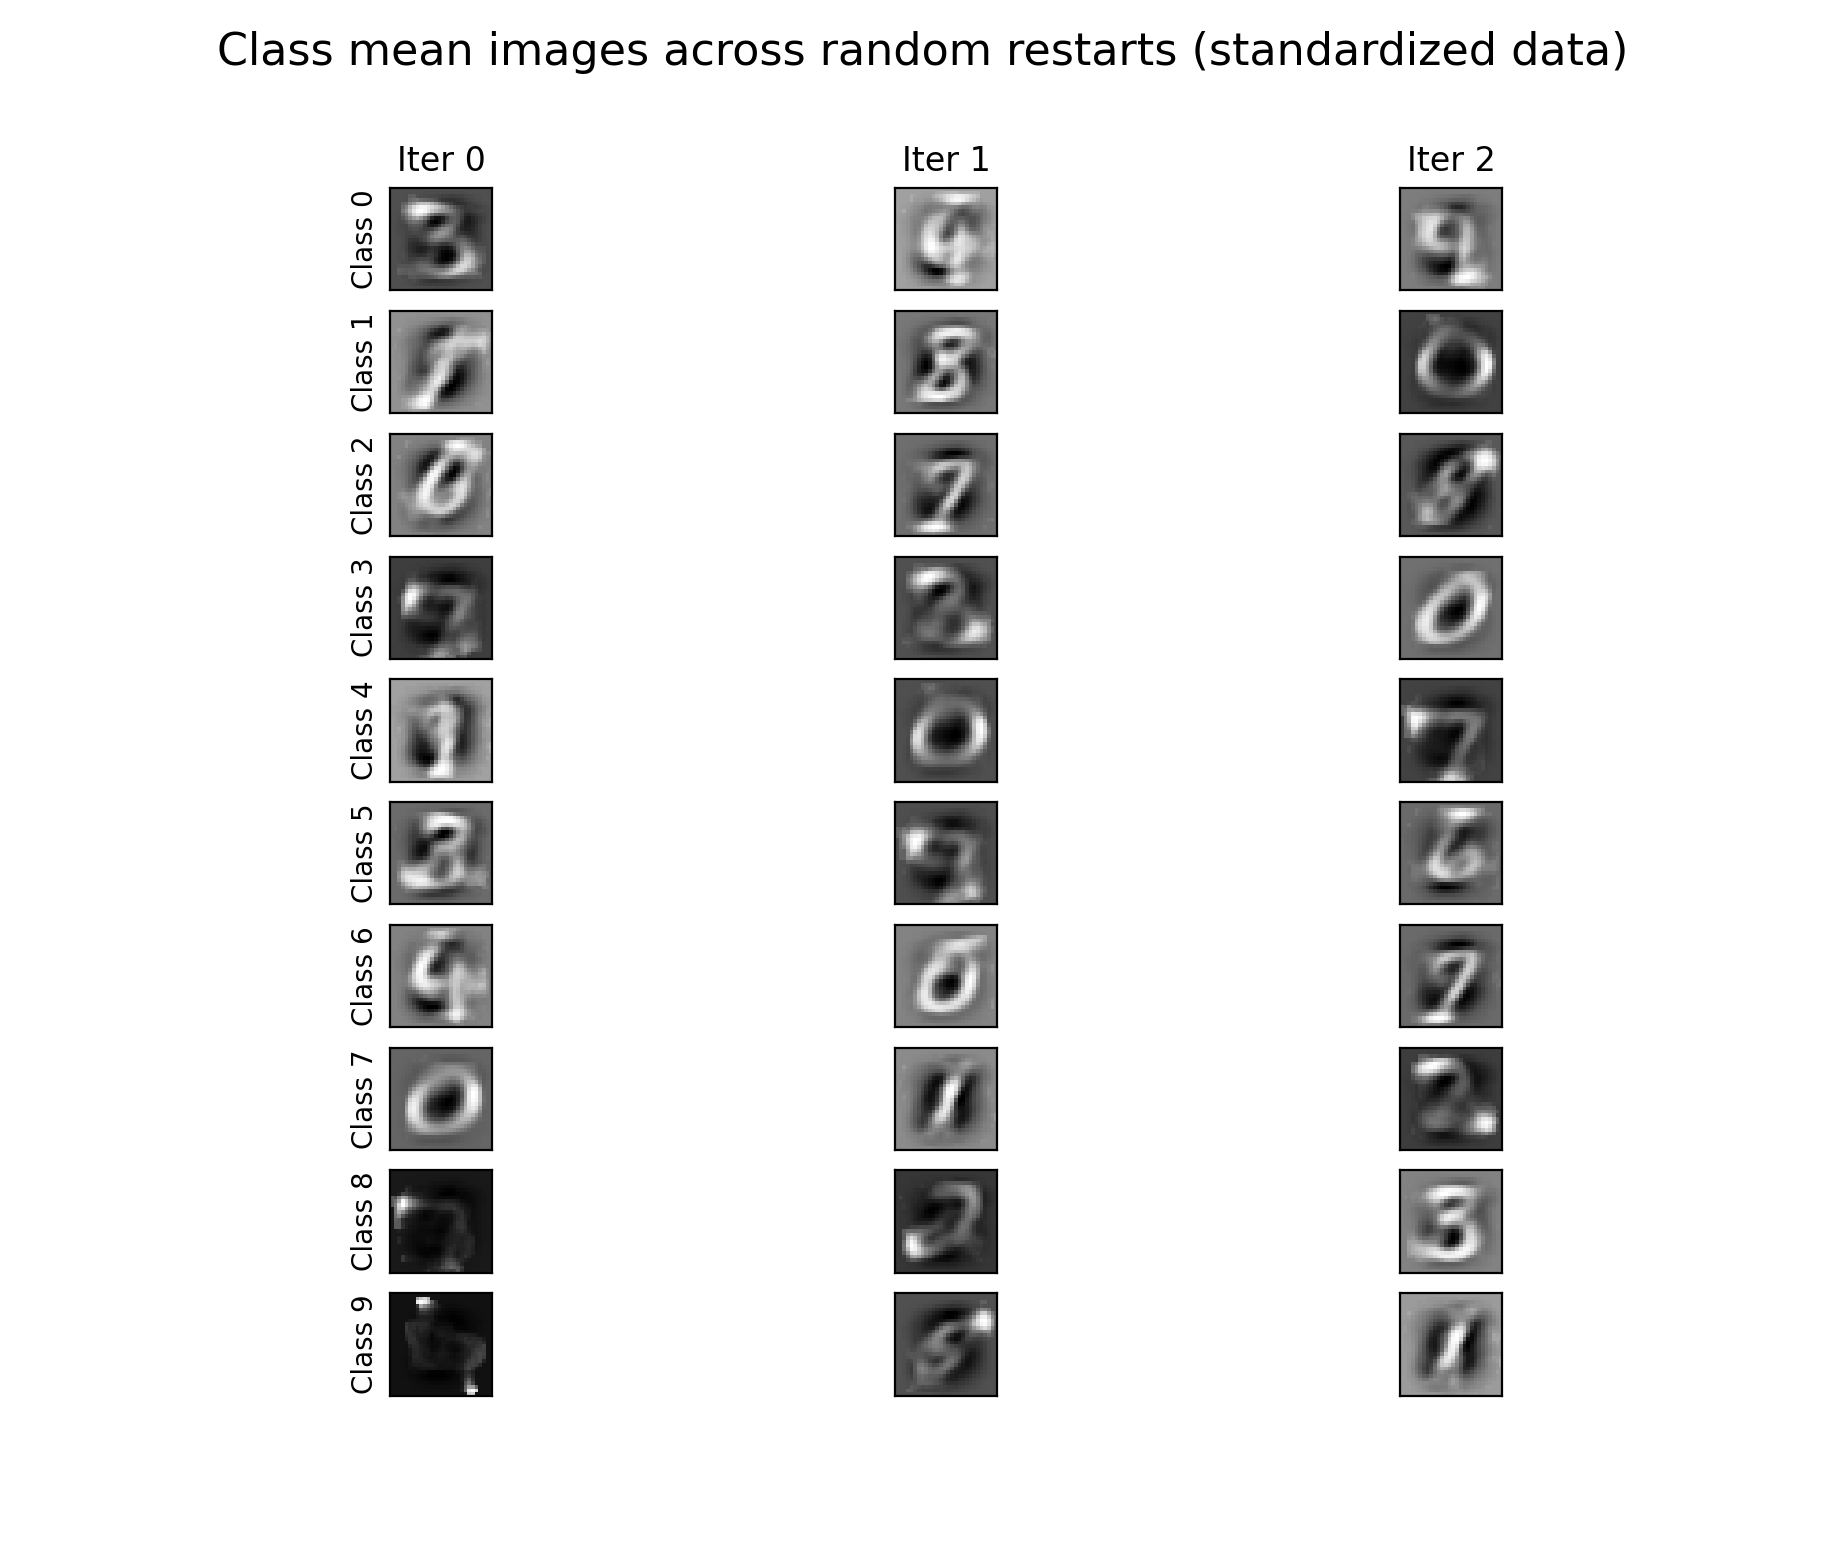
\includegraphics[scale=0.5]{plots/kmeans-standardized.png}

The centroids are quite different from the non-standardized K-means from 2.2. In the standardized centroids, the edges of each mean image are much lighter and more grey, whereas only the centers of the images show a contrast between white and black. I think the higher contrast in the center is due to the tendency for the centers to have higher variance than the edges: this causes them to still be either starkly white are black, as opposed to the edges which remain a more neutral grey.

\newpage
\subsection*{2.4}
We want to implement HAC for min, max, and centroid-based linkages, then display the mean image for 10 clusters on a single plot.

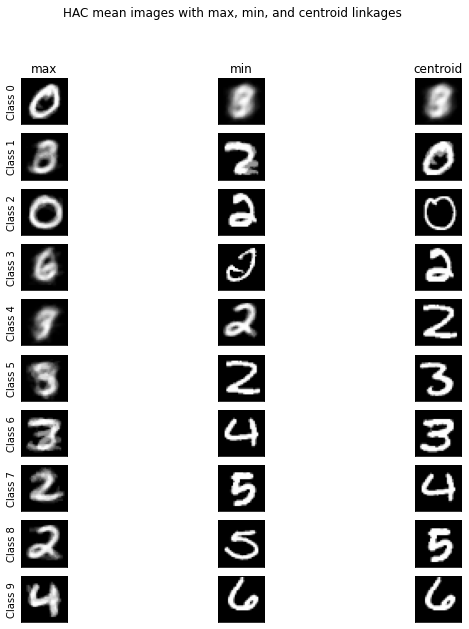
\includegraphics[scale=0.5]{plots/hac.png}

The cluster means for centroid and min linkages are much crisper than that of our k-means for the most part, with only one of the images in the min and centroid linkage being quite blurry. However, the max linkage looks fairly similar to the k-means linkage in terms of crispness / bluriness.

We only run HAC once because it is deterministic and so there is no need to run it multiple times because it would always produce the same result.

\newpage
\subsection*{2.5}

We want to plot the number of images in each cluster for HAC with max, min, and centroid-based linkages, as well as a run of our k-means.

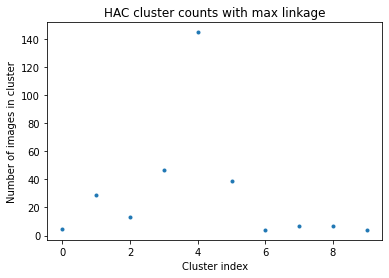
\includegraphics[scale=0.5]{plots/hacmax-clusters.png} \
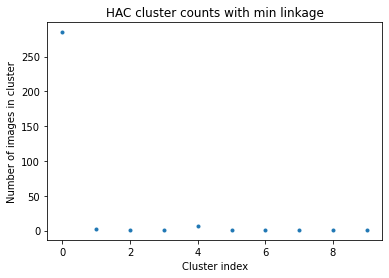
\includegraphics[scale=0.5]{plots/hacmin-clusters.png}

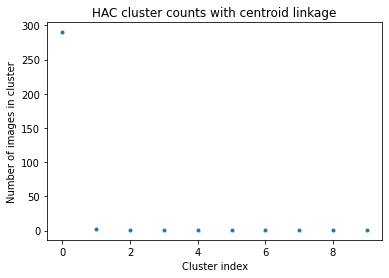
\includegraphics[scale=0.5]{plots/haccentroid-clusters.png} \
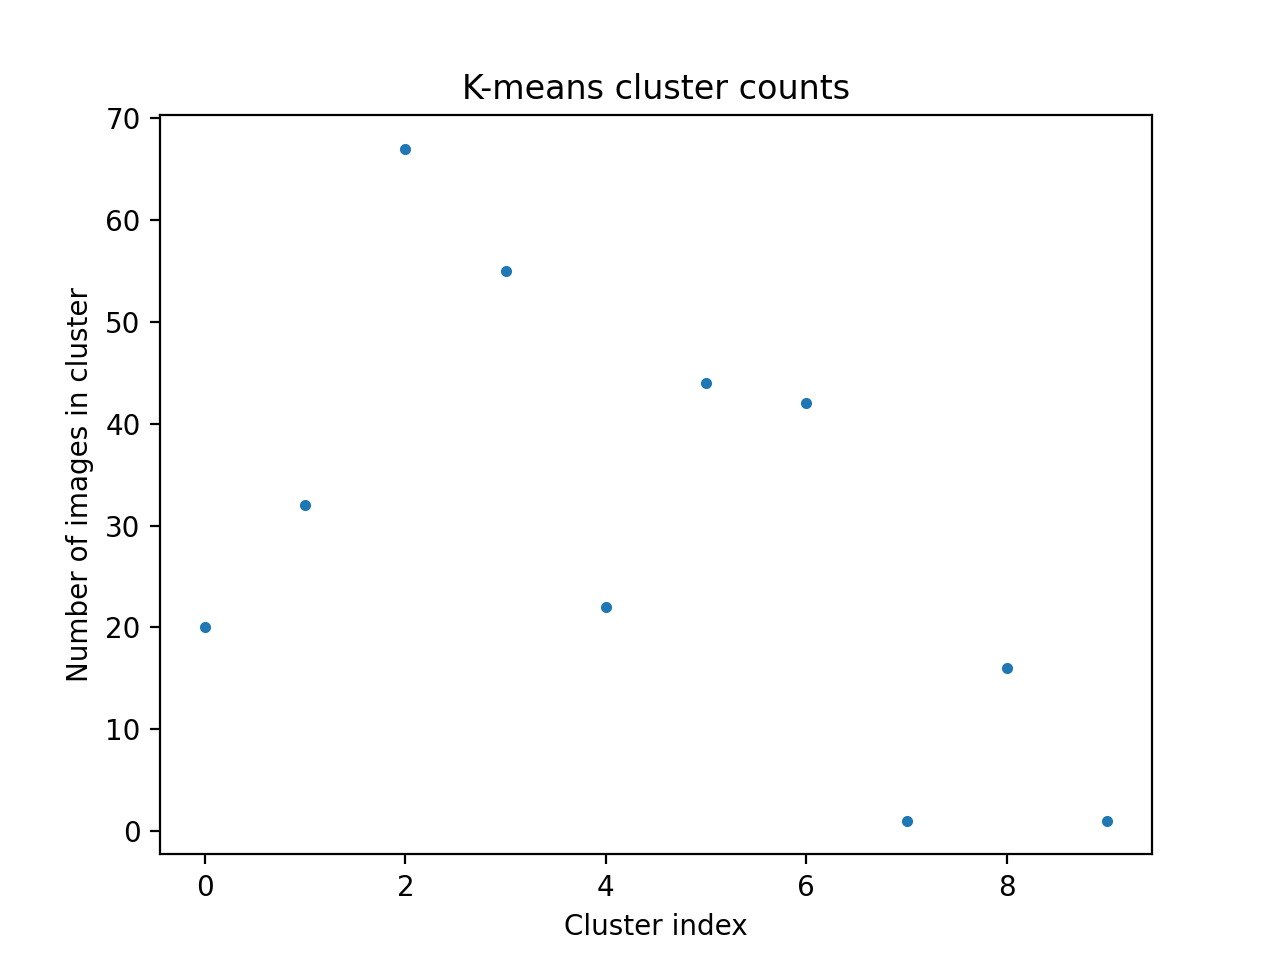
\includegraphics[scale=0.44]{plots/kmeans-clusters.png}

Intuitively, this suggests that min linkage tends to have one cluster with many perhaps less similar images that ``snake'' through the data (since the min linkage takes the closest cluster at each step), whereas the max linkage tends to have more evenly divided clusters that are perhaps more ``blobby'' and similar within each cluster.

This helps explain the crispness and blurriness of some of the clusters. For the min and centroid linkage, most clusters only have a few very similar images, while one image takes on many images and thus most of the variation in the images. The max linkage is more similar to k-means because the max linkage has more uniform clusters and so is blurrier.

\newpage
\subsection*{2.6}
We want to plot a confusion matrix between each pair of HAC min/max/centroid and K-means with $K = 10$ models.

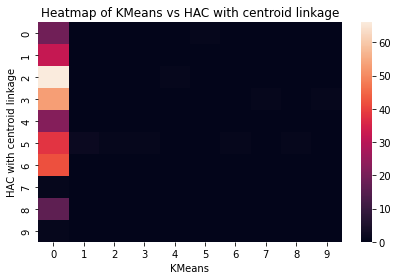
\includegraphics[scale=0.5]{plots/kmeans-haccentroid.png} \
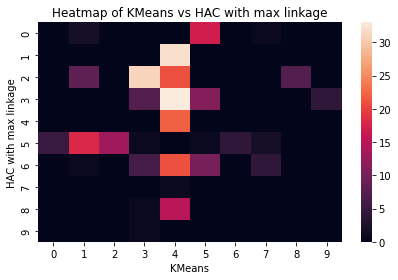
\includegraphics[scale=0.5]{plots/kmeans-hacmax.png}

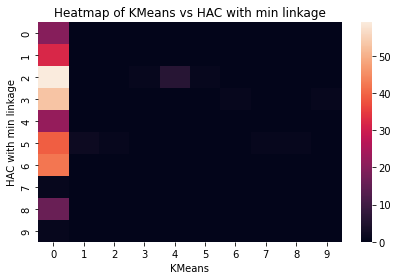
\includegraphics[scale=0.5]{plots/kmeans-hacmin.png} \
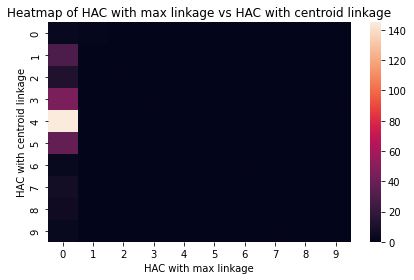
\includegraphics[scale=0.5]{plots/hacmax-haccentroid.png}

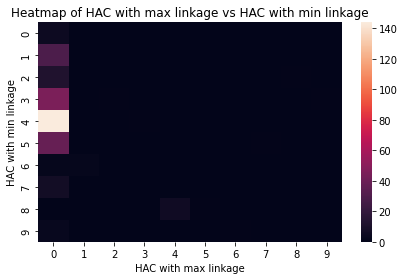
\includegraphics[scale=0.5]{plots/hacmax-hacmin.png} \
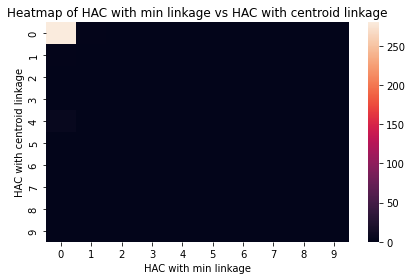
\includegraphics[scale=0.5]{plots/hacmin-haccentroid.png}

The HAC with max linkage is closest to k-means. This may be because the clusters are more uniformly sized with the max-linkage and so there is a higher likelihood of overlap between the clusters in k-means. Moreover, this may be because the max linkage has a more similar effect to the k-means objective function. A max linkage effectively ``punishes'' clusters that are far apart more heavily than min and centroid linkages, since it takes the smallest maximum distance between clusters: if there are two points that are very far apart between the clusters, then HAC will not merge those two clusters unless it absolutely must. This is similar to k-means, which uses a squared distance to assign points to the means. This similar effect causes more overlap between the clusters in HAC with max linkage and k-means and so a more similar confusion matrix.

\newpage
\subsection*{2.7}

I think that computing the confusions for each clustering to the true digit labels is not a reasonable evaluation metric for the clustering. Since clustering is an unsupervised learning technique, its primary aim is to explore underlying trends and structures in the data as opposed to supervised learning which focuses on predicting the label of a new data given previous data. So using the true digit labels would not be aligned with the primary aim of clustering. Additionally, since clustering focuses on grouping data that looks similar (based off a distance function), using this metric ignores possible complications in the data. For example, suppose that all images of $4$'s and $9$'s look quite similar in the MNIST data, but there are two styles to draw $1$'s that are very different. This could cause a clustering model to group $4$'s and $9$'s together and the different styles of $1$'s in different clusters, since the distance between the $4$ and $9$ images is smaller than the distance between the different styles of $1$. This is expected behavior of the clustering model, but would cause the metric to perform very badly in an unreasonable way. Thus this metric is not reasonable.


\newpage
%%%%%%%%%%%%%%%%%%%%%%%%%%%%%%%%%%%%%%%%%%%%%
% Problem 3
%%%%%%%%%%%%%%%%%%%%%%%%%%%%%%%%%%%%%%%%%%%%%

\begin{problem}[Ethics Assignment, 5pts]

Select a real-life outcome in Artificial Intelligence or Machine Learning 
that you believe is morally wrong. You can select your own outcome from 
the news or select one of the outcomes in the options below:

\begin{itemize}
    \item COMPAS, a case management tool predicting recidivism that 
        flagged “blacks are almost twice as likely as whites to be 
        labeled a higher risk but not actually re-offend” (Angwin 
        2016).
        
    \item An NLP algorithm filled in the inference “Man is to 
        \_\_\_\_ as woman is to \_\_\_\_” with “Man is 
        to computer programmer as woman is to homemaker” (Bolukbasi 
        et al, 2016).
        
    \item \url{http://www.survivalofthebestfit.com/game}: a game that 
        exemplifies algorithmic bias in resume screening
        
    \item IBM Diversity in faces: insufficient training data for 
        darker-skinned faces
        
    \item Other Unfair Algorithms: Algorithms of Oppression (a really 
        good book with tons of examples), VI-SPDAT, Allegheny Family 
        Screening Tool
        
\end{itemize}
Draw a causal chain that resulted in this outcome and circle the choice points that were the largest contributors to the outcome. At each morally relevant choice point, write two alternative decisions that could have prevented the outcome.

\end{problem}

\newpage
\subsection*{Solution}
For this problem, I chose the game \url{http://www.survivalofthebestfit.com/game} and to create a causal chain for some of its outcomes.

\includegraphics[scale=0.5]{causal-chain.png}

I think that the two most morally relevant choice points are proceeding to automate hiring, and to do nothing after noticing deficiencies with the model. These are highlighted in red. I think that automating hiring is a backward-looking responsibility: I should have raised concerns and not made this decision. In many ways, this decision was the primary enabler for the outcome. I think that not shutting down the model is both a backward and a forward looking responsibility: while I should have shut down the model earlier, I have a responsibility to shut it down now, and put the cat back in the bag.

\newpage
%%%%%%%%%%%%%%%%%%%%%%%%%%%%%%%%%%%%%%%%%%%%%
% Name and Calibration
%%%%%%%%%%%%%%%%%%%%%%%%%%%%%%%%%%%%%%%%%%%%%
\subsection*{Name}

\subsection*{Collaborators and Resources}
Whom did you work with, and did you use any resources beyond cs181-textbook and your notes?\\
James Kitch, Julian Schmitt
\\
Did you attend office hours for help with this homework?
No.

\subsection*{Calibration}
Approximately how long did this homework take you to complete (in hours)? 
20

\end{document}